\subsection{User Trust} \label{sec:trust}
    In designing assurances that affect trust-based user behaviors, it is critical to know what drives those behaviors. Because of this, some time must be spent to understand what trust is. 

    Trust is critical in interpersonal relationships, and it affects the dynamics of intelligent multi-agent systems as simple as one-on-one personal interactions  \cite{Lewicki2006-hj}, to more complicated ones such as financial markets and governments \cite{Fukuyama1995-un}. Consequently, researchers in psychology, sociology, and economics have historically sought to understand the fundamental principles of trust, each with the aim of understanding their field better \cite{Gambetta1988-pi}. Moral philosophers have also thought intently about the topic \cite{Baier1986-im}.

    Due to wide interest spanning many disciplines it is difficult, if not impossible, to write a succinct definition of trust that would appease all interested parties. Besides that, trust is actually a very broad concept that evades precise definitions at a high level. However the following definition, adapted from \cite{McKnight2004-vv}, is broad enough to avoid too much contention:

    \begin{description}
        \item [Trust:] a psychological state in which an agent willingly and securely becomes vulnerable, or depends on, a trustee (e.g., another person, institution, or an AIA), having taken into consideration the characteristics (e.g., benevolence, integrity, competence) of the trustee.
    \end{description}

    \subsubsection{Trust between AIAs and humans?}
        Trust is generally understood to exist between people. Is it possible for a human to enter into a trusting relationship with an AIA?
        % In their paper regarding important human factors that should be considered when designing autonomous machines \cite{Sheridan1984-kx} are seemingly the first to discuss the idea that trust relationships between humans and autonomous systems are important, and to suggest that humans need some assurance that the ``commands will be carried out properly''. They also mention the idea that ``there needs to be an accurate perception of [the autonomous system's] trustworthiness''. Finally they suggest that ``appropriate criteria for trust need to be studied to develop a theory of trust in supervisory control''.
        % Perhaps motivated by \citeauthor{Sheridan1984-kx}\cite{Sheridan1984-kx}, a few years later \cite{Muir1987-mk}, and later in more detail \cite{Muir1994-ow}, create a psychologically based model of trust that considered the ``component expectations of trust'' of \cite{Barber1983-yc} and the dynamic evolution of trust from \cite{Rempel1985-sg}, to make a framework for studying trust in human-machine relationships.
        % \citet{Muir1996-gt} reported the results of two experimental studies to investigate the validity of her proposed model. She claims that these were the first experiments to explicitly ask "operators to rate their trust in automated equipment", and to see if they could do so under normal operating conditions. She found that operators were able to rate their trust in the automation, and that the level of trust changed based on different performance characteristics of the automated system. In her own words: "These results suggest that operators' subjective ratings of trust and the properties of the automation which determine their trust, can be used to predict and optimize the dynamic allocation of functions in automated systems".
        That humans actually do feel trust towards machines has been experimentally confirmed several times in research using common subjective psychological questionnaires. Some examples include: \citet{Muir1996-gt,Reeves1997-ad,Groom2007-bz,Mcknight2011-gv,Riley1996-qm,Bainbridge2011-pl,Kaniarasu2012-mo,Salem2015-md,Desai2012-rc, Freedy2007-sg, Wang2016-id, Inagaki1998-cl, Kaniarasu2013-ho}. 

        Several academic experiments have investigated the possibility of trust existing between humans and (according to the terminology of this survey) AIAs. All found that some level of trust can be formed in such relationships. For instance, \citet{Lacher2014-yc} points out that people trust an AIA at different levels. For example, an operator would have different perspectives on trust based on their level of interaction with the AIA. The designer of an AIA would also trust the AIA differently than an end user, due to the differing nature of the trust relationship from one to the other. 
        % \citet{Lankton2008-ct} claims, and finds some support for the idea, that trust in technology is fundamentally different from interpersonal trust between humans. They demonstrate the validity of the hypothesis by using a survey of 427 college students regarding Facebook. However, the authors point out that this study was based on a single set of survey data about facebook, and may not be unbiased or apply to other technologies. Beyond this, it is the author's opinion that the `fundamental differences' they point out are not that divergent from the human-human trust model.

        \citet{Tripp2011-cq} investigate the variation of trust between humans and different levels of technology. They run experiments with three different levels of technology: Microsoft Access, a recommender system, and Faceobook. They found that `human-like' trust applied more to Facebook, while `system-like' trust applied more to MS Access. They conclude that if the system is `human enough', then a human trust model is appropriate.

        Given this research, we will take the position of presenting a human-human trust model and use it as a basis for human-AIA trust -- with the understanding that the strength of the model varies with the complexity of the AIA. In other words, some features of the model will have varying level of significance over the range of adaptability and capability of AIAs.

\subsubsection{A Model of Human-AIA Trust}
        We now present a model of human-AIA trust, which will cast insights on assurances that will be discussed later. It should be noted that this model is being presented as \emph{one possible model} that can be helpful in understanding assurances -- it is neither the only model, or a perfect model. As research advances, such models will likely continue to evolve, and the ideas of assurances will naturally evolve as well.
            % This has been recently attempted in the context of human-AIA relationships \cite{Lahijanian2016-nd}, but with an overly simplistic reduction of trust. The reality is that trust is extremely complex, and so dealing with it in the setting of human-AIA relationships is going to be complex.

        In work relating to business management, \citet{McKnight1998-ty}, and later \citet{McKnight2001-fa}, performed what is, arguably, the first multi-disciplinary survey and unification of trust literature, which also condensed it into a single typology. The resulting model is shown, with some minor adaptations, in Figure \ref{fig:UserTrust}. The figure illustrates the three categories that make up a human's trust. There are causal arrows that connect the different components. The `Dispositional Trust' block is generally considered by psychologists, and deals with long-term psychological traits that develop in a person from childhood. The `Instututional Trust' block is generally studied by sociologists, and represents the level to which a person trusts social/commercial structures. Finally, the `Interpersonal Trust' block is deals directly with one-on-one relationships and can generally fluctuate more quickly than the other two.

        \begin{figure}[htbp]
            \centering
            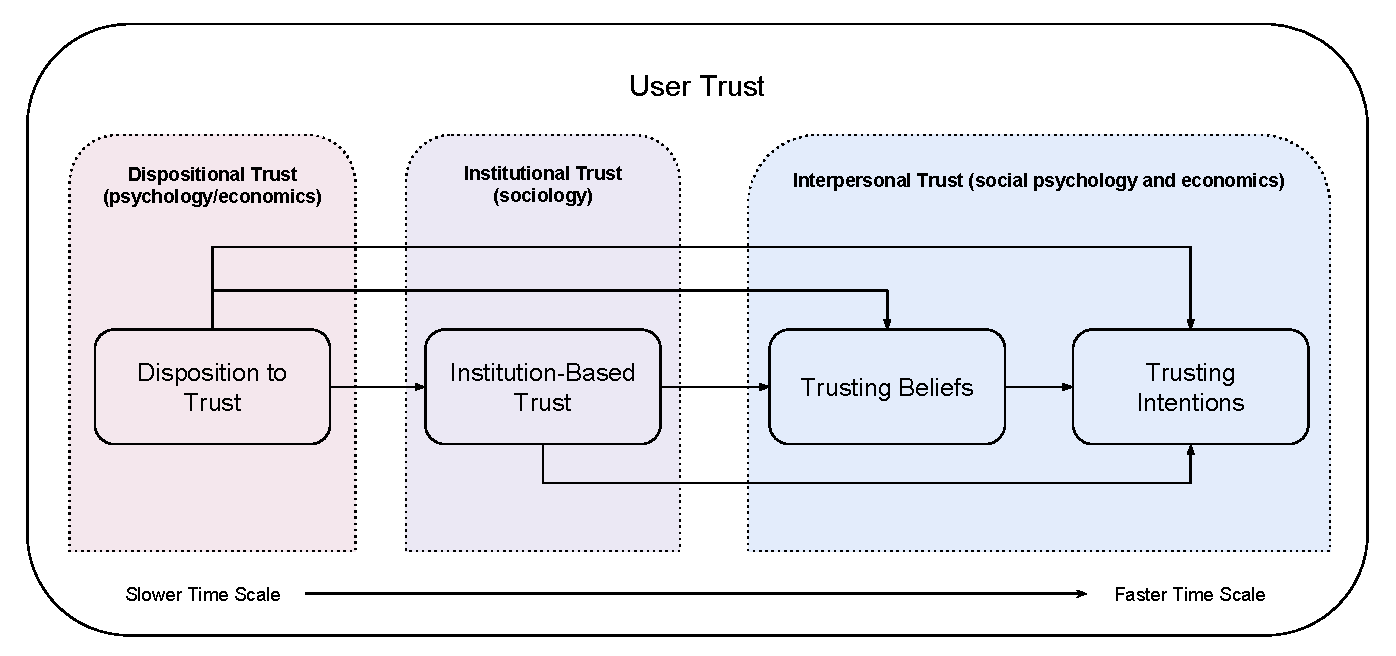
\includegraphics[width=0.9\textwidth]{Figures/UserTrust}
            \caption{Interdisciplinary trust model proposed by \citet{McKnight2001-fa}. The three main categories are delineated, and corresponding disciplines that are interested are listed within parentheses. Connections indicate a causal relationship.}
            \label{fig:UserTrust}
        \end{figure}

        In the context of AIAs the components of the three categories from figure \ref{fig:UserTrust} are defined as follows:

        \begin{description}
            \item [Disposition to Trust:] The extent to which one displays a consistent tendency to be willing to depend on AIAs in general across a broad spectrum of situations and persons
            \item [Institution-Based Trust:] One believes that regulations are in place that are conducive to situational success in an endeavor
            \item [Trusting Beliefs:] One believes that the AIA has one or more characteristics beneficial to oneself
            \item [Trusting Intentions:] One is willing to depend on, or intends to depend on, the AIA even though one cannot control its every action
        \end{description}

        Each of these main categories of trust has components defined in Figure \ref{fig:Assurance_classes}. These components were defined through the compilation of many research studies across research disciplines, and because of this represent the most accurate notion of the components of trust available. It is asserted here that these are the principal drivers of TRBs, the components at which assurances are targeted, and way in which assurances can be classified.

        \begin{sidewaysfigure}[htbp]
            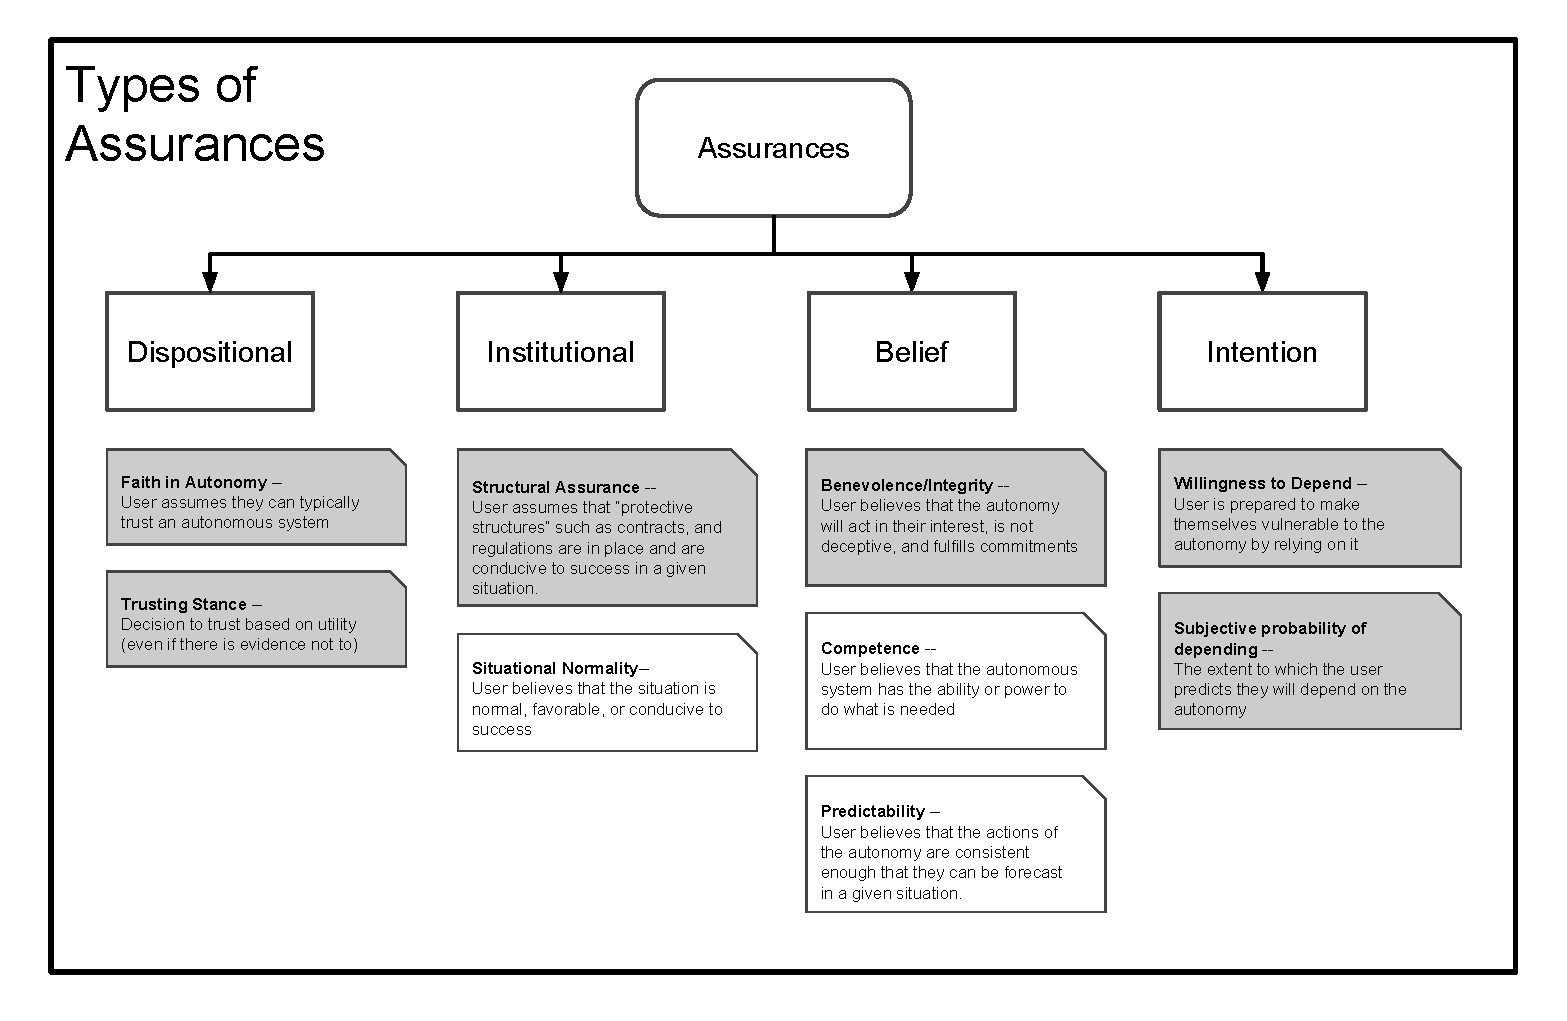
\includegraphics[width=8in]{Figures/Assurances.pdf}%
            \caption{Classification of assurances based on the component definitions of the main categories of trust: `Disposition to Trust', `Institution-Based Trust', `Trusting Beliefs', and `Trusting Intentions'}
            \label{fig:Assurance_classes}
        \end{sidewaysfigure}
